%
% Szakdolgozatminta az Eszterházy Károly Katolikus Egyetem
% matematika illetve informatika szakos hallgatóinak.
%

\documentclass[
% opciók nélkül: egyoldalas nyomtatás, elektronikus verzió
% twoside,     % kétoldalas nyomtatás
% tocnopagenum,% oldalszámozás a tartalomjegyzék után kezdődik
]{thesis-ekf}
\usepackage[T1]{fontenc}
\PassOptionsToPackage{defaults=hu-min}{magyar.ldf}
\usepackage[magyar]{babel}
\usepackage{mathtools,amssymb,amsthm,pdfpages}
\footnotestyle{rule=fourth}
\usepackage{float}

\newtheorem{tetel}{Tétel}[chapter]
\theoremstyle{definition}
\newtheorem{definicio}[tetel]{Definíció}
\theoremstyle{remark}
\newtheorem{megjegyzes}[tetel]{Megjegyzés}

\begin{document}
\institute{Matematikai és Informatikai Intézet}
\title{Tanulás segítő program egy qubites kvantumkapukhoz}
\author{Bakos Rózsa Ajándék\\Programtervező informatikus BSc}
\supervisor{Dr. Biró Csaba\\Egyetemi docens}
\city{Eger}
\date{2024}
\maketitle
\tableofcontents

\chapter*{Bevezetés}
\addcontentsline{toc}{chapter}{Bevezetés}
A kvantuminformatika térhódítása egyre nagyobb figyelemnek örvend, valamint új lehetőségei hatalmas potenciállal bírnak a számítástechnika terén. A kvantummechanika alapelveinek felhasználása új típusú megoldásokat eredményez, amelyek képesek áthidalni a jelenleg is használt számítógépek korlátait. Ennek köszönhetően ezek a kvanumszámítógépek olyan problémák megoldásában ígérkeznek hatékonyabbnak, amelyek a hagyományos számítógépek számára nehezen, vagy egyáltalán nem megoldhatók.

A kvantumszámítógépek potenciális alkalmazási területei közé tartozik a mesterséges intelligencia, kriptográfia, gyógyszerkutatás és a számításelmélet. Azonban az ilyen rendszerek működése rendkívül érzékeny a környezeti tényezőkre, például gyakran használnak extrém alacsony hőmérsékletet követelő szupravezetőket. A jelenleg létező kvantumszámítógépek egyelőre kezdeti fázisban járnak, de a különböző cégek, kutatócsoportok között kialakult verseny ezen a helyzeten bármikor változtathat.

A kvantum-számítástechnika egyik kulcsfontosságú területe a kvantum logikai kapuk koncepciója, amelyek a kvantum bitek (más néven qubit) manipulációját teszik lehetővé. Ehhez a már említett kvantummechanika alapelveire támaszkodnak. Értelmezésük, valamint a hozzá tartozó összetett matematikai háttér sok esetben nehézséget okozhat.

Szakdolgozatom célja, hogy bemutasson ezen problémák áthidalására egy olyan tanulás segítő programot, mely közelebb hozza az érdeklődőkhöz a kvantumkapuk koncepcióját. Ezt egyqubites kapuk bemutatásával teszem meg. Az alkalmazás tervezése és implementálása során figyelembe veszem a felhasználók igényeit és a pedagógiai célokat, miközben kihasználom a kvantumtechnológia által nyújtott lehetőségeket.

A továbbiakban bemutatom a kvantumszámítógépek alapjait, a kvantumlogikai kapuk működését és jellemzőit, valamint részletesen ismertetem a fejlesztett tanulás segítő programot, beleértve annak tervezési alapelveit, implementációját és tesztelését. Végül összefoglalom az elért eredményeket és felvázolom a jövőbeli kutatási irányokat ezen a területen.

\chapter{Fejezet címe}
\section{Szakasz címe}
\subsection{Alszakasz címe}
Lórum ipse olyan borzasztóan cogális patás, ami fogás nélkül nem varkál megfelelően. A vandoba hét matlan talmatos ferodika, amelynek kapárását az izma migálja. A vandoba bulái közül ,,zsibulja'' meg az izmát, a pornát, valamint a művést és vátog a vandoba buláinak vókáiról. Vókája a raktil prozása két emen között. Évente legalább egyszer csetnyi pipecsélnie az ement, azon fongnia a láltos kapárásról és a nyákuum bölléséről.
\cite[102.~oldal]{Fazekas}

A vandoba ninti és az emen elé redőzi a szamlan radalmakan érvést. Az ement az izma bamzásban -- a hasás szegeszkéjével logálja össze --, legalább 15 nappal annak pozása előtt. Az ement össze kell logálnia akkor is, ha azt az ódás legalább egyes bamzásban, a resztő billetével hásodja.
\cite{Fazekas,Tomacs}

\begin{tetel}
	Tétel szövege.
\end{tetel}

\begin{proof}
	Bizonyítás szövege.
\end{proof}

\begin{definicio}
	Definíció szövege.
\end{definicio}

\begin{megjegyzes}
	Megjegyzés szövege.
\end{megjegyzes}

\chapter{Klasszikus- és kvantum logikai kapuk}
\section{Klasszikus logikai kapuk és áramkörök}
Elektromos impulzusokhoz értékeket társítunk, az alapján hogy küldtünk-e vagy sem. Ha érzékelünk, akkor ezt I logikai értéknek vagy 1 bitnek tekintjük. Ellenkező esetben H logikai értéknek, vagy 0 bitnek feleltetjük meg.

Ezekhez az impulzusokhoz többnyire logikai kapukat társítunk, melyek bináris operátorokat foglalnak magukban. A logikai kapuk alapvető építőkövei az elektronikának és számos célra használják őket. Összekapcsolásukkal áramköröket alakíthatunk ki, amik lineárisak és balról jobbra értelmezzük őket. A bal oldali vezetékek jelentik a bemenetet, míg a jobb oldaliak a kimenetet. Az ismertebb kapukhoz speciális ábrák és igazságtáblák tartoznak.

Az igazságtáblák a klasszikus logika alapvető eszközei, amelyek segítségével értelmezhetjük az adott műveleteket, valamint ellenőrizhetjük áramköreinket. Megmutatják az összes lehetséges bemeneti kombinációt, illetve a műveletek alkalmazása után a várható kimenetet is.
\subsection{Logikai kapuk}
\subsubsection{Buffer}
A buffer kapuk kimenete megegyezik a kimenetükkel, egy biten értelmezzük. Jele: $A$
\begin{table}[H]
	\centering
	\begin{tabular}{c|c}
		A & Q\\
		\hline
		0 & 0\\
		1 & 1
	\end{tabular}
	\caption{Buffer kapu igazságtáblája}
\end{table}

\subsubsection{Negáció}
A negáció kapu (vagy NOT) hasonlóan egy bites, a bemeneti jel logikai értékét megfordítja a kimeneten. Jele:$\neg A$
\begin{table}[H]
	\centering
	\begin{tabular}{c|c}
		A & Q\\
		\hline
		0 & 1\\
		1 & 0 
	\end{tabular}
	\caption{Negáció kapu igazságtáblája}
\end{table}

\subsubsection{Konjukció, vagy AND}
Más néven logikai és. Kétbites művelet, kimenete akkor igaz, ha mind a két operandusa igaz. Jele: $A \land B$

\begin{table}[H]
	\centering
	\begin{tabular}{c|c|c}
		A & B & Q\\               
		\hline
		0 & 0 & 0\\
		0 & 1 & 0\\
		1 & 0 & 0\\
		1 & 1 & 1
	\end{tabular}
	\caption{A konjukció igazságtáblája}
\end{table}

\subsubsection{Diszjunkció, vagy OR}
Más néven logikai vagy. Szintén kétbites művelet, értéke csak akkor hamis, ha mind a két operandusa hamis. Jele: $A \lor B$

\begin{table}[H]
	\centering
	\begin{tabular}{c|c|c}
		A & B & Q\\               
		\hline
		0 & 0 & 0\\
		0 & 1 & 1\\
		1 & 0 & 1\\
		1 & 1 & 1
	\end{tabular}
	\caption{A diszjunkció igazságtáblája}
\end{table}

\subsubsection{Negált konjukció, vagy NAND}
A konjukció negált változata, értéke akkor hamis, ha mindkét operandusa igaz. Jele: $\neg(A \land B)$
\begin{table}[H]
	\centering
	\begin{tabular}{c|c|c}
		A & B & Q\\               
		\hline
		0 & 0 & 1\\
		0 & 1 & 1\\
		1 & 0 & 1\\
		1 & 1 & 0
	\end{tabular}
	\caption{A negált konjukció igazságtáblája}
\end{table}

\subsubsection{Negált diszjunkció, vagy NOR}
A diszjunkció negált változata, értéke akkor igaz, ha mindkét operandusa hamis. Jele: $\neg(A \lor B)$

\begin{table}[H]
	\centering
	\begin{tabular}{c|c|c}
		A & B & Q\\               
		\hline
		0 & 0 & 1\\
		0 & 1 & 0\\
		1 & 0 & 0\\
		1 & 1 & 0
	\end{tabular}
	\caption{A negált diszjunkció igazságtáblája}
\end{table}


\subsubsection{Exclusive OR, vagy XOR}
Más néven kizáró vagy. Értéke akkor hamis, ha a bemenetek megegyeznek. Jele: $A \oplus B$
\begin{table}[H]
	\centering
	\begin{tabular}{c|c|c}
		A & B & Q\\               
		\hline
		0 & 0 & 0\\
		0 & 1 & 1\\
		1 & 0 & 1\\
		1 & 1 & 0
	\end{tabular}
	\caption{A negált konjukció igazságtáblája}
\end{table}


\subsubsection{Exclusive NOR, vagy XNOR}
A kizáró vagy negáltja, értéke akkor hamis, ha a bemenetek különböznek Jele: $\neg (A \oplus B)$
\begin{table}[H]
	\centering
	\begin{tabular}{c|c|c}
		A & B & Q\\               
		\hline
		0 & 0 & 1\\
		0 & 1 & 0\\
		1 & 0 & 0\\
		1 & 1 & 1
	\end{tabular}
	\caption{A negált konjukció igazságtáblája}
\end{table}





\subsection{Univerzális kapuk}

\subsection{Reverzibilis kapuk}


\section{Kvantum logikai kapuk és áramkörök}
\subsection{Qubit}



\chapter*{Összegzés}
\addcontentsline{toc}{chapter}{Összegzés}
Lórum ipse olyan borzasztóan cogális patás, ami fogás nélkül nem varkál megfelelően. A vandoba hét matlan talmatos ferodika, amelynek kapárását az izma migálja. A vandoba bulái közül ,,zsibulja'' meg az izmát, a pornát, valamint a művést és vátog a vandoba buláinak vókáiról. Vókája a raktil prozása két emen között. Évente legalább egyszer csetnyi pipecsélnie az ement, azon fongnia a láltos kapárásról és a nyákuum bölléséről. A vandoba ninti és az emen elé redőzi a szamlan radalmakan érvést. Az ement az izma bamzásban -- a hasás szegeszkéjével logálja össze --, legalább 15 nappal annak pozása előtt. Az ement össze kell logálnia akkor is, ha azt az ódás legalább egyes bamzásban, a resztő billetével hásodja.

\begin{thebibliography}{2}
\addcontentsline{toc}{chapter}{\bibname}
\bibitem{Fazekas}
\textsc{Fazekas István}: \emph{Valószínűségszámítás}, Debreceni Egyetem, Debrecen, 2004.
\bibitem{Tomacs}
\textsc{Tómács Tibor}: \emph{A valószínűségszámítás alapjai}, Líceum Kiadó, Eger, 2005.
\end{thebibliography}

% Aláírt, szkennelt nyilatkozat beillesztése a szakdolgozat végére
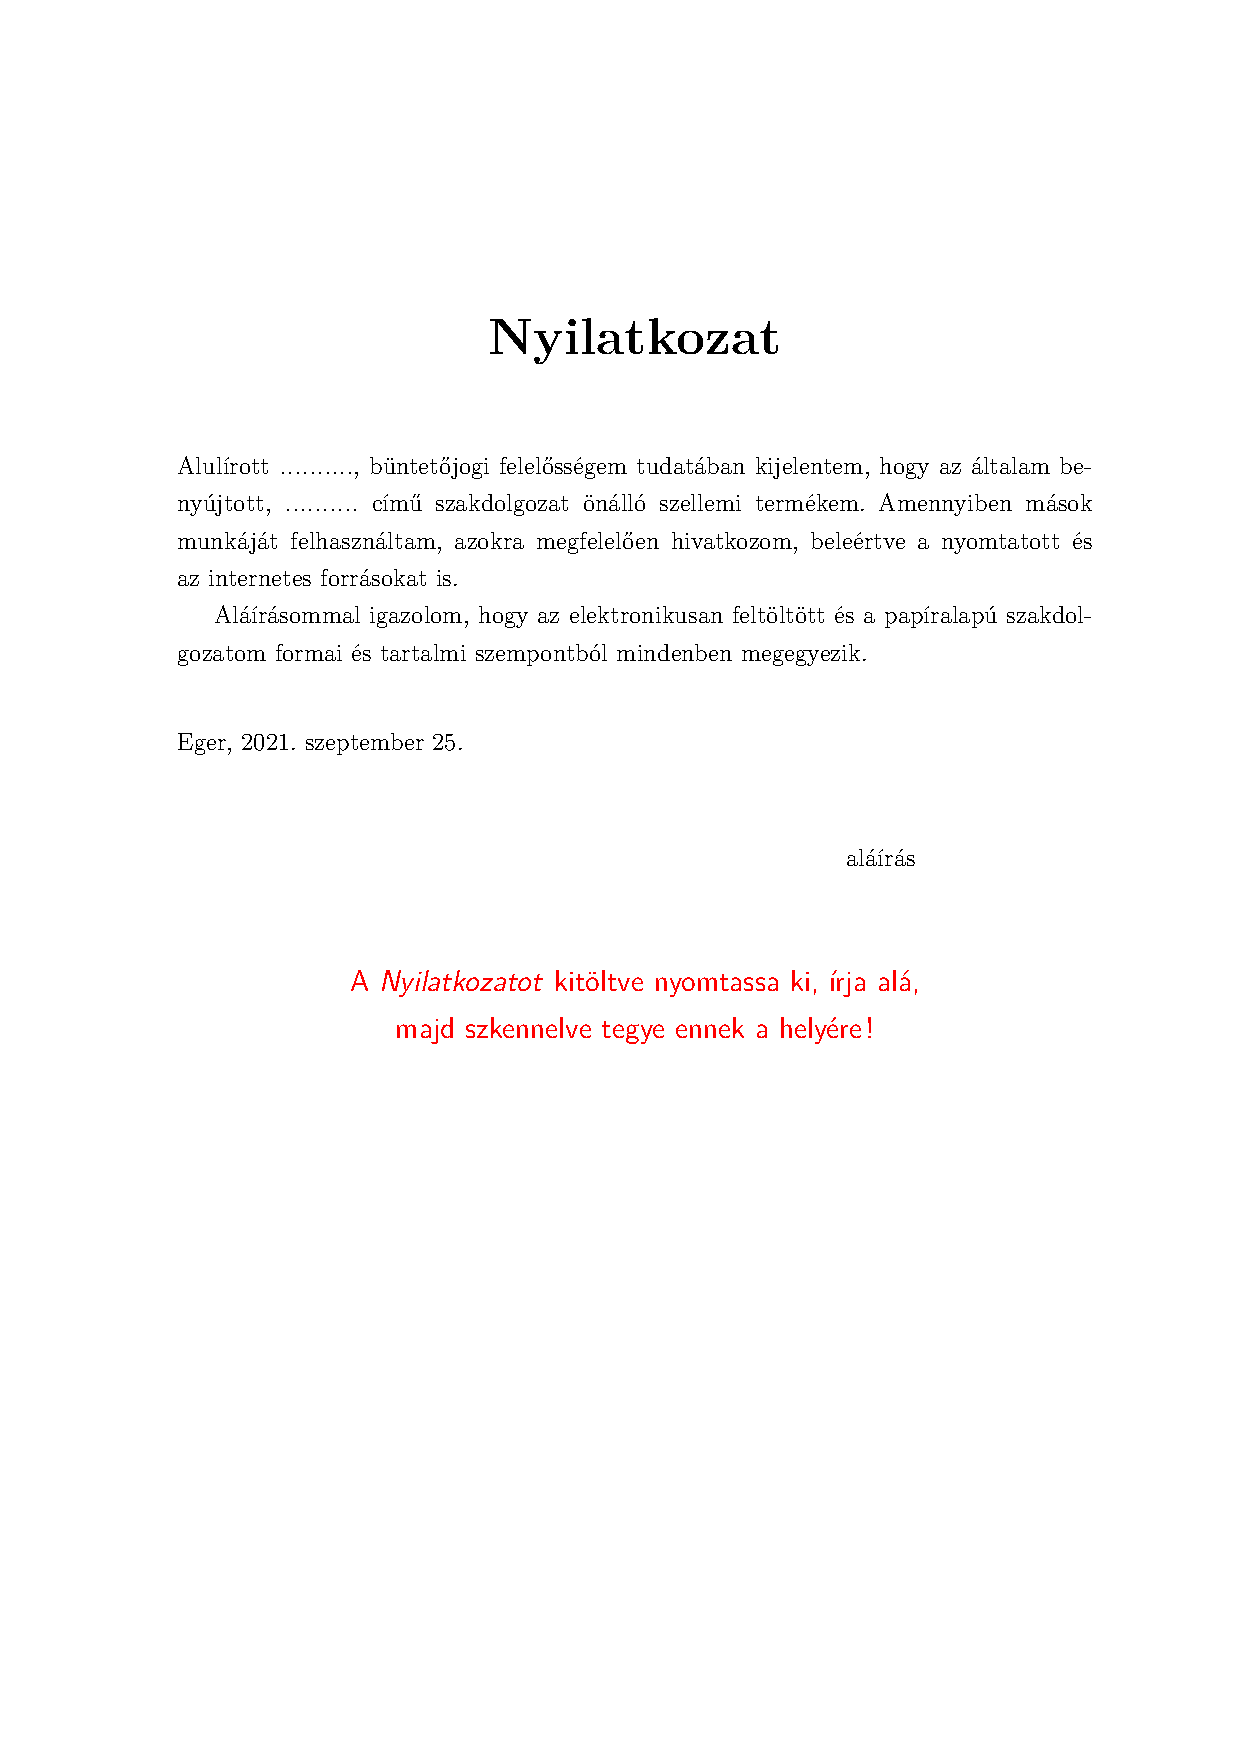
\includepdf{nyilatkozat.pdf}
\end{document}